\documentclass[finnish]{tktltiki2}% {{{

% --- General packages ---

\usepackage[utf8]{inputenc}
\usepackage[T1]{fontenc}
\usepackage{lmodern}
\usepackage{microtype}
\usepackage{amsfonts,amsmath,amssymb,amsthm,booktabs,color,graphicx}
\usepackage[pdftex,hidelinks]{hyperref}
% Automatically set the PDF metadata fields
\makeatletter
\AtBeginDocument{\hypersetup{pdftitle = {\@title}, pdfauthor = {\@author}}}
\makeatother

% --- Language-related settings ---
%
% these should be modified according to your language

% babelbib for non-english bibliography using bibtef
\usepackage[fixlanguage]{babelbib}
\selectbiblanguage{finnish} 
% {{{

% add bibliography to the table of contents
\usepackage[nottoc]{tocbibind}
% tocbibind renames the bibliography, use the following to change it back
\settocbibname{Lähteet}

% --- Theorem environment definitions ---

\newtheorem{lau}{Lause}
\newtheorem{lem}[lau]{Lemma}
\newtheorem{kor}[lau]{Korollaari}

\theoremstyle{definition}
\newtheorem{maar}[lau]{Määritelmä}
\newtheorem{ong}{Ongelma}
\newtheorem{alg}[lau]{Algoritmi}
\newtheorem{esim}[lau]{Esimerkki}

\theoremstyle{remark}
\newtheorem*{huom}{Huomautus}

\def\figureautorefname{kuva}

% --- tktltiki2 options ---
%
% The following commands define the information used to generate title and
% abstract pages. The following entries should be always specified:
\title{Samanaikaisuus verkkopalvelinsovelluksessa}
\author{Vili Lipo}
\date{\today}
\level{Kandidaatin tutkielma}
\abstract{Tässä tutkielmassa vertaillaan verkkopalvelimien suunnittelumalleja
  ja niiden suorituskykyä. Verkkopalvelin on ohjelma, joka vastaa useiden asiakkaiden pyyntöihin
  verkkosivuilla tai verkkosovelluksissa. Pyyntöihin vastaamiseen
  voi liittyä laskentaa, tietokantaoperaatioita tai muita toimenpiteitä.

Vertailuun valittiin Reactor/Proactor-malli, säiereservimalli, SYMPED-malli ja SEDA-malli.
Tavoitteena on selvittää millä mallilla voidaan
edistää verkkopalvelinsovelluksen suorituskykyä parhaiten.
Vertailussa otetaan huomioon myös se, kuinka 
valittu suunnittelumalli vaikuttaa sovelluslogiikan
kehittämisen haastavuuteen. Vertailun kolmas näkökulma
on miten valittu suunnittelumalli vaikuttaa verkkopalvelinsovelluksen
vakauteen.
}

% The following can be used to specify keywords and classification of the paper:

\keywords{palvelin, tapahtumaohjattu, samanaikaisuus}

% classification according to ACM Computing Classification System (http://www.acm.org/about/class/)
% This is probably mostly relevant for computer scientists
% uncomment the following; contents of \classification will be printed under the abstract with a title
% "ACM Computing Classification System (CCS):"
\classification{Software and its engineering $\rightarrow$ Software organization and properties
$\rightarrow$ Software system structures $\rightarrow$ Distributed systems organizing principles}

% If the automatic page number counting is not working as desired in your case,
% uncomment the following to manually set the number of pages displayed in the abstract page:
%
% \numberofpagesinformation{16 sivua + 10 sivua liitteissä}
%
% If you are not a computer scientist, you will want to uncomment the following by hand and specify
% your department, faculty and subject by hand:
%
% \faculty{Matemaattis-luonnontieteellinen}
% \department{Tietojenkäsittelytieteen laitos}
% \subject{Tietojenkäsittelytiede}
\begin{document}
\frontmatter      % roman page numbering for front matter

\maketitle        % title page
\makeabstract     % abstract page

\tableofcontents  % table of contents

% --- Main matter ---

\mainmatter       % clear page, start arabic page numbering

% }}}
\section{Johdanto}
Verkkopalvelinsovelluksien suorituskyky vaikuttaa vahvasti
Internetin välityksellä käytettävien palveluiden käyttökokemukseen ja toimivuuteen.
Verkkopalvelimien taakat ovat vaihtelevia, joten
yleispätevän verkkopalvelimen tulisi skaalautua saatavilla oleviin resursseihin.
Jos verkkopalvelimen käyttötarkoitus ei ole suorittaa laskennallisesti raskaita
tehtäviä, sen
kriittisimmät resurssit ovat I/O-resurssit.

Verkkopalvelimen tehokkuuteen ja skaalautumiseen vaikuttaa olennaisesti
sen suunnittelumalli. Tässä
tutkielmassa vertaillaan eri suunnittelumalleja palvelimen toimintojen samanaikaistamiseen.
Kirjallisuudessa suunnittelumallista käytetään myös nimeä palvelinarkkitehtuuri.

Samanaikaisessa ohjelmassa ohjelman osat ovat näennäisesti samaan
aikaan suorituksessa, mutta todellisuudessa ne suoritetaan peräkkäin.
Käyttöjärjestelmä jakaa suoritusaikaa ohjelman eri osille,
ja vuorottelemalla antaa ihmisnäkökulmasta vaikutelman samanaikaisuudesta.

Rinnakkaisuudella tarkoitetaan tietojenkäsittelytieteessä useiden
eri operaatioiden suorittamista järjestelmässä samaan aikaan useilla suorittimilla.
Kun suorittimia
on useita, käyttöjärjestelmä pystyy aikatauluttamaan toimintoja
rinnakkain ja näin kaksi ohjelman osaa on todellisesti
samalla hetkellä suorituksessa.

Verkkopalvelimen suunnittelumalli on osa palvelinsovellusta,
joka on mielekästä toteuttaa moduulina tai kirjastona.
Näin palvelimen sovelluslogiikka voidaan irrottaa rinnakkaisuutta
käsittelevästä logiikasta. Yleispätevät
samanaikaisuutta käsittelevät rakenteet voidaan sitten
käyttää uudelleen toisissa projekteissa.
Tavoitteena on selvittää mikä suunnittelumalli edistää
parhaiten verkkopalvelinsovelluksen suorituskykyä ja
kehitystyötä.

Vertailussa perehdytään säiereservimalliin (threadpool-model), Reactor-malliin\cite{schmidt_reactor:_1995} ja sen jatkokehityksiin
kuten Proactor-malliin~\cite{hu_applying_1998}, SYMPED-malliin ja SEDA-malliin~\cite{welsh_seda_2001}.
Vertailun keskeisimmät kriteerit ovat suorituskyky, vakaus ja
sovelluslogiikan kehittämiseen liittyvät haasteet.

Verkkopalvelinsovelluksen suorituskyky ja skaalautuvuus
määrittävät palvelun laadun raskaan kuormituksen aikana.
Poikkeus-ja virhetilanteet vaikuttavat hyvin negatiivisesti
palvelun laatuun. Jos poikkeustilanne johtaa
palvelun kaatumiseen, voivat seuraamukset olla vakavat
palvelun ylläpitäjän ja asiakkaiden kannalta.
Palvelimen suunnittelumalli voi vaikuttaa 
sovelluskohtaisen logiikan kehittämiseen.
Jos malli tekee kehitystyöstä hyvin haastavaa,
kehitystyön kustannukset nousevat.
Suunnittelumallin tulisikin edistää
samanaikaisuutta ja rinnakkaisuutta vaikeuttamatta
sovelluslogiikan kehitystä.

Vertailun perusteella voidaan todeta, että
yksinkertaisuudestaan huolimatta tehokkailla asynkronisilla
kutsuilla varustettu Reactor-mallinen verkkopalvelinsovellus
kykenee vastaamaan suurenkin palvelun tarpeisiin, jos palvelun
pullonkaula on I/O-operaatiot~\cite{schmidt_reactor:_1995}.
Proactor-mallilla~\cite{hu_applying_1998} voidaan tarjota kehittäjille edistyneempiä työkaluja
asynkronisten operaatioiden hallintaan.

Säiereservimallin on hyvä vaihtoehto, jos palvelimen
toimintaan liittyy enemmän laskentaa ja sen tehokkuus ei ole I/O-sidonnainen.
Laskennallisesti raskaaseen palvelimeen voidaan myös soveltaa SEDA-mallia~\cite{welsh_seda_2001}.
Siinä pyyntöjen käsittely jaetaan eri tasoille ja tasojen käsittelyyn
hyödynnetään säiereservejä.

Tapahtumanohjatun mallin voi laajentaa moniprosessimallia noudattavaksi,
jos sen skaalautuvuus ei muuten riitä.
Yhdistämällä Reactor-tai Proactor-mallinen palvelin säireserviin
saadaan SYMPED-mallinen palvelin, jolla tapahtumaohjatusta palvelimesta
saadaan paremmin skaalautuva moniprosessorijärjestelmissä.

Luvussa~\ref{vps} kerrotaan taustatietoa asiakas-palvelin-mallista, palvelinympäristöstä
ja rinnakkaisuudesta.
Luvussa~\ref{sec:SM} esitellään verkkopalvelimien suunnittelumalleja. Luvussa~\ref{sec:vertailu}
malleja vertaillaan ja analysoidaan. Luvussa~\ref{sec:yhteenveto} on yhteenveto aiheesta.

\section{Verkkopalvelinsovellus}\label{vps}

Tässä luvussa kerrataan
asiakas-palvelin-malli, palvelinympäristö ja rinnakkaisuuden keskeiset käsitteet.
Verkkopalvelinsovellus on osa internetsivuston tai palvelun tarjoavaa
asiakas-palvelin-mallin toteutusta. 
Sen tehtävä on vastata internetsivuston tai palvelun toteuttamiseen
liittyviin pyyntöihin eli lähettämään tietyn HTTP-pyynnön
perusteella oikea HTML-tiedosto~\cite{Berners-Lee_1994},
tekstimuotoinen datatiedosto, tai kuvatiedosto.
Asiakas-palvelin-mallin jälkeen esitetään
HTTP-protokollan perustoiminta ja REST-rajapinnan yleiset periaatteet.


Verkkopalvelinsovelluksen suorituskyvyn kannalta
on tärkeää hyödyntää laitteiston resurssit mahdollisimman hyvin.
Käyttöjärjestelmä toimii ympäristössä rajapintana
laitteistolle ja vaikuttaa suuresti resurssien
käyttämiseen. Laitteiston useiden
suorittimien hyödyntämiseen sovelluksessa tarvitaan useita
prosesseja tai säikeitä, jolloin käyttöjärjestelmä
pystyy aikatauluttamaan niitä kaikilla suorittimilla.

Samanaikaisuuteen ja rinnakkaisuuteen liittyy
ohjelmointiongelmia, joiden kertaaminen
auttaa hahmottamaan paremmin tutkielmassa
esitettäviä suunnittelumalleja. Ongelmista
oleellisimpia on kilpailutilanteet ja lukkiutuminen.
Luvun kolmannessa osassa
keskitytään näihin ongelmiin.

\subsection{Asiakas-palvelin-malli}
Asiakas-palvelin-mallissa
asiakasohjelma tarjoaa käyttäjälle käyttöliittymän sovellukseen. Palvelinohjelma
tarjoaa määritellyn rajapinnan
palveluita asiakasohjelmalle verkkoyhteyden yli~\cite{sinha_client-server_1992}.
Tieto välittyy ohjelmien välillä pyyntöinä ja vastauksina ja näin palvelinohjelma ja
asiakasohjelma
muodostavat löysästi yhdistetyn järjestelmän.

Asiakasohjelma siis yhdistää käyttöliittymässä tapahtuvat toimet palvelimen
rajapinnan pyynnöiksi. Se voi hyödyntää pyyntöjen tulosten tallentamista
muistiin. Näin tarvittavia pyyntöjä voidaan vähentää, käyttämällä
paikallisesta muistista löytyviä vastauksia.
Asiakasohjelma voi myös suorittaa
laskentaa tai muita toimenpiteitä paikallisesti~\cite{sinha_client-server_1992}.

Asiakasohjelmat voivat olla työpöytäsovelluksia, jotka hyödyntävät käyttöjärjestelmän
ikkunointi-ja käyttöliittymäominaisuuksia~\cite{sinha_client-server_1992}.
Tämänkaltaisen asiakasohjelman toteuttamisessa voidaan käyttää mitä tahansa ohjelmointikieltä,
ja asiakasohjelman toiminnallisuutta voi laajentaa lähes rajatta.

Asiakasohjelma voi olla myös verkkosivu. 2000-luvun alussa
pelkkään HTML-standardiin perustuvat verkkosivut pystyivät
tarjoamaan käyttöliittymiä esimerkiksi keskustelualustoille ja verkkokaupoille.
Näissä järjestelmissä valtaosa suorittamisesta on palvelimen vastuulla,
sillä sen pitää tiedonkäsittelemisen lisäksi kirjoittaa tieto
esitettävään HTML-muotoon käyttöliittymän näkymäksi. Palvelin
siis vastaa selaimen pyyntöön lähettämällä kokonaisen HTML-tiedoston.

HTML-näkymät voivat olla valmiina tiedostojärjestelmässä eli staattisia tai
palvelin voi täydentää merkkauskielellä kirjoitettuun pohjaan
tietoja tietokannasta tai muusta sovelluksen tilatiedosta. 
Tilatietoa käyttäviä näkymiä kutsutaan dynaamisiksi sivuiksi~\cite{pai_flash_1999}.

Nykyisten selaimien JavaScript suoritustuen ansiosta yhä
monimutkaisempia asiakasohjelmia voidaan toteuttaa
selaimella saavutettavilla verkkosovelluksina.
Nykyään palvelimen ja asiakkaan
välisessä tiedonvälityksessä on muodikasta käyttää REST-rajapintaa, jossa
yksittäisen dataresurssin saavuttaminen on helppoa~\cite{battle_bridging_2008}.
Asiakasohjelma pyytää vain haluamansa resurssit, ja ne saatuaan piirtää
niiden pohjalta
itsenäisesti käyttöliittymän näkymän.

Palvelin tarjoaa sen rajapinnan määrittämiä palveluita asiakasohjelmille.
Palvelin ei itsenäisesti aloita yhteyttä mihinkään
asiakkaisiin vaan se odottaa niiden pyyntöjä.
Se pystyy palvelemaan useita asiakkaita, jopa
eri asiakasohjelmia, kunhan asiakasohjelmat noudattavat
palvelimen rajapintaa~\cite{sinha_client-server_1992}.
Palvelimen palvelut muodostavat järjestelmän keskeisen
sovelluslogiikan, jossa asiakaspyynnön parametreilla
suoritetaan toimintoja ja palvelin lähettää
tuloksen vastauksena~\cite{sinha_client-server_1992}.

Yleisesti palvelin vastaa järjestelmän turvallisuudesta~\cite{sinha_client-server_1992} sillä,
sen toiminnan vääristäminen on haastavampaa paha-aikeisille
toimijoille, kun taas asiakasohjelman toiminnan muuntelu on suoraviivaisempaa.
Asiakasohjelmaa ajetaan laitteella, joka ei ole verkkosovelluksen
ylläpitäjän hallussa. Paha-aikeiset toimijat voivat käyttää tätä hyväkseen
ja tarkkailla asiakasohjelman lähettämiä pyyntöjä tai sen
suorituskäyttäytymistä kuten resurssien käyttöä.
Tarkkailusta selvinneiden tietojen avulla on mahdollista
kiertää asiakasohjelmaan toteutettuja suojauksia.

Palvelinohjelman toimintaa vääristääkseen
paha-aikeisten toimijoiden tulisi päästä
käsiksi sitä suorittavan järjestelmän hallintatoimintoihin, tai
löytää haavoittuvuus sen rajapinnasta. Näin mahdollisuuksia
toteuttaa hyökkäys on huomattavasti vähemmän kuin sovelluksella, jota
suoritetaan hyökkääjien omalla laitteistolla.

Palvelin vastaa myös tunnistautumisesta ja käyttöoikeuksien hallinnasta~\cite{pai_flash_1999}.
Monen palvelun toteuttamisen kannalta on kriittistä, että
tiedon käyttöoikeuksia voidaan rajata käyttäjän tunnistautumisen perusteella.

Yksinkertainen esimerkki asiakas-palvelin-mallista on tietokantapalvelin,
jossa tietokannan tiedot on tallennettu palvelimelle. Tietokantapalvelimelta
voidaan asiakasohjelmalla tehdä verkkoyhteyden läpi tietokantakyselyitä. Asiakasohjelma
voi sitten suorittaa laskentaa tietokannan tiedoilla.

HTTP-protokollaa~\cite{leach_hypertext} käytetään verkkopalvelinsovelluksien ja
asiakasohjelmien väliseen viestintään verkon sovellustasolla.
HTTP-protokollan tärkeitä termejä on yhteys, viesti, pyyntö ja vastaus.
Yhteydellä tarkoitetaan virtuaalista yhteyttä, jonka asiakas ja palvelin muodostavat.
HTTP-versioon 1.1 lisättiin pysyvät yhteydet, joilla pyritään
vähentämään yhteyden muodostamiseen tarvittavia pyyntöjä ja paketteja verkon
käytössä. Versiosta 1.1 eteenpäin pysyvät yhteydet ovat protokollan
oletuskäytöstä. Yhteys suljetaan, jos asiakas tai palvelin lähettää
viestin, jossa on käsky sulkea yhteys~\cite{leach_hypertext}.

HTTP-protokolla on pyyntö-vastaus protokolla~\cite{leach_hypertext}. Asiakas lähettää
verkon yli palvelimelle pyynnön, joka sisältää metodin, URI-osoitteen, protokollan
version, MIME-tyyppisen viestin, asiakasinformaation ja mahdollisesti
sisältöä. Palvelin puolestaan vastaa statusrivillä, jossa on protokollan
versionumero ja onnistumis-tai virhekoodi, MIME-tyyppinen viesti palvelimen
tiedoista ja metatiedosta, jota seuraa mahdollisesti sisältöä.
Internettiä selatessa selain lähettää vierailtavien verkkosivujen
palvelimille HTTP-GET-pyyntöjä, joihin palvelimet vastaavat
lähettämällä verkkosivua vastaavan HTML-tiedoston.

REST~\cite{battle_bridging_2008} on HTTP-protokollan
päälle rakennettu suunnittelutekniikka verkkopalveluiden mallintamiseen.
Siinä jokaista sovelluksen dataresurssia vastaa URI-osoite,
jonka polkuun kuuluu dataresurssin tunnistetieto.
REST:in keskiössä on joukko tilanmuutos\-operaatioita,
jotka ovat yleisiä mille tahansa tietojärjestelmälle. 
Nämä operaatiot ovat: luo, lue, päivitä ja poista.
Niihin viitataan yleensä englanninkielisellä
akronyymillä CRUD.
Näitä operaatioita voi kohdistaa dataresursseihin
HTTP-pyynnöillä resurssien yksilöiviin URI-osoitteisiin.

\subsection{Palvelinympäristö}
Verkkopalvelinsovelluksen ympäristön keskeisiä
tekijöitä ovat laitteisto, käyttöjärjestelmä ja sovellus itse.
Verkkopalvelinsovellus ja käyttöjärjestelmä
yrittävät yhteistyössä hyödyntää laitteistoa
mahdollisimman tehokkaasti.

Käyttöjärjestelmän tehtävä on hallinnoida laitteistoa.
Verkkopalvelinsovellus käyttää käyttöjärjestelmän
tarjoamia rajapintoja laitteiston hyödyntämiseksi.
Verkkopalvelinsovellukselle tärkeitä
käyttöjärjestelmän tehtäviä on 
prosessien ja säikeiden aikataulutus ja I/O-resurssien hallinta.

Verkkopalvelimia suoritetaan laitteistoilla, joilla
on jopa kymmeniä suorittimia. Käyttöjärjestelmä
aikatauluttaa suorituksessa olevia ohjelmia näiden välillä.
Ohjelmien aikatauluttamiseen liittyy prosessit ja säikeet.
Prosessi on yksi ohjelma tai osa ohjelmaa, joka on suorituksessa järjestelmässä.
Sen suoritustilatiedot ja tunniste on
tallennettu käyttöjärjestelmässä prosessin kuvaajaan~\cite{stallings_operating_2018}.
Jokaisella
prosessilla on oma muistialue ja prosessien välinen kommunikaatio
tapahtuu ainoastaan käyttöjärjestelmän tarjoamien
rajapintojen läpi~\cite{stallings_operating_2018}.

Prosessin kuvaajaan tallennettujen arvojen avulla käyttöjärjestelmä
voi suorittaa useaa ohjelmaa samanaikaisesti, kun käyttöjärjestelmän
vuoronantaja jakaa prosesseille suoritusaikaa. Kun prosessi vaihtuu
käyttöjärjestelmä asettaa suorittimen suoritusympäristöksi
uuden prosessin kuvaajaan tallennetun ympäristön. Tätä kutsutaan kontekstin
vaihdoksi. Vanhan prosessin suoritinympäristö puolestaan talletetaan sen
kuvaajaan~\cite{stallings_operating_2018}.

Nykyisissä käyttöjärjestelmissä voi prosessin suoritusta jakaa usealle
säikeelle. Prosessissa on silloin yksi tai useampia säikeitä.
Säikeet jakavat prosessin muistialueen ja tiedostoresurssit.
Säikeiden kuvaajiin
tallennetaan niiden suoritustilatieto,
kuten rekisterien ja pinon arvot~\cite{stallings_operating_2018}.

Koska säikeisiin liittyy vähemmän tietoa, kuin prosesseihin,
on niiden luominen ja tuhoaminen nopeampaa. Säikeiden välinen
kommunikointi on myös huomattavasti nopeampaa kuin prosessien, koska
ne voivat välittää tietoa jakamansa muistialueen läpi.
Prosessit voivat kommunikoida keskenään vain käyttöjärjestelmän
avulla~\cite{stallings_operating_2018}.
Suorituksessa olevan säikeen
vaihdossa suoritinympäristö pitää vaihtaa
samaan tapaan kuin prosessienkin kohdalla, mutta muistirajoitteisessa
järjestelmässä keskusmuistissa olevia
tietoja ei tarvitse vaihtaa, sillä saman prosessin säikeet jakavat
muistin.

ydintasonsäikeet ovat säikeitä joiden aikatauluttamisesta vastaa
käyttöjärjestelmän ydin. Käyttäjätason säikeet ovat sellaisia säikeitä,
joiden aikatauluttamisesta vastaa jokin käyttäjätason ohjelma kuten
säiekirjasto. Käyttäjätason aikatauluttamisen puutteista johtuen
kaksi saman prosessin käyttäjätason säiettä ei voi olla suorituksessa
samaan aikaan~\cite{stallings_operating_2018}. 

Tiedonsiirtäminen eri laitteiden välillä on verkkopalvelinsovelluksen
ydintoimintaa~\cite{pai_flash_1999}.
Tämän takia verkkopalvelinsovellukselle erityisen tärkeitä resursseja ovat
I/O-resurssit.
Verkkopalvelinsovellus suorittaa pääasiassa verkko-ja levy-I/O:ta~\cite{pai_flash_1999}.
Käyttöjärjestelmä vastaa I/O-operaatioiden toteuttamisesta,
jotta I/O:n käyttäminen sovelluksissa on samanlaista
riippumatta laitteistosta.

Verkko-I/O on toimintaa, jossa ohjelma käyttää tietokoneen
verkkosovitinta kommunikoidakseen verkon muiden laitteiden kanssa.
Verkkopalvelinsovellus käyttää verkko-I/O:ta lukiessaan
asiakkaan pyyntöjä ja kirjoittaessaan HTTP-otsakkeen ja
vastauksen asiakkaalle~\cite{pai_flash_1999}.
Laitteiston verkkoliikennekapasiteetilla kuvataan maksimimäärää bittejä tietyllä aikavälillä,
jonka verkko tai verkkosovitin on kykenee siirtämään laitteen ja verkon muiden laitteiden välillä.
Verkkopalvelinsovellus voi olla yhteydessä tietokantapalvelimeen
verkonvälityksellä ja suorittaa tietokantakyselyitä verkko-I/O:n läpi.
Kun palvelimen kuormitus on suuri, sen tulisi pystyä hyödyntämään
sen verkkoinfrastruktuuria tehokkaasti korkealla käyttöasteella. Eli
pyyntöjen vastaanottamisen ja vastauksien lähettämisen käyttäisi
lähes koko verkkoliikennekapasiteettia.

Levy-I/O:lla tarkoitetaan tiedon siirtämistä
tietokoneen keskusmuistin ja massamuistin välillä.
Verkkopalvelinsovellus käyttää levy-I/O:ta lukiessaan
asiakkaan pyyntöihin liittyviä tiedostoja tiedostojärjestelmästä~\cite{pai_flash_1999}.
Luettavat tiedostot voivat olla valmiita HTML-tiedostoja tai täytettäviä
pohjia, jotka täytetään sovelluksen tilatiedon perusteella ennen
asiakkaalle lähettämistä.

I/O-operaatiot vievät tietokoneen mittakaavassa paljon
aikaa~\cite{pai_flash_1999}. Estävässä I/O-operaatiossa säie tai prosessi,
joka kutsuu I/O-operaatiota suorittaa I/O:n itse.
Estävät kutsut aiheuttavat suorituskykyongelmia, jos
I/O-resurssi ei ole vapaa, kun sovellus kutsuu sitä.
Tässä tilanteessa käyttöjärjestelmä muuttaa sovelluksen
tilan suorittaa tilasta odottaa tilaan~\cite{stallings_operating_2018}.
Sovelluksen suoritus
siis keskeytyy kokonaan, kunnes I/O-laite vapautuu ja käyttöjärjestelmä
herättää sovelluksen.
Estävät kutsut ovat kuitenkin kehittäjälle yksikertaisia, sillä
ne ovat luonteeltaan aivan tavallista peräkkäistä
koodia.

Odottaa tilaan joutumista voi välttää tarkastamalla
I/O-laitteen vapauden ennen operaation suorittamista~\cite{schmidt_reactor:_1995}.
Jos
I/O-laite on vapaa, I/O-operaatio suoritetaan. Jos I/O-laite
ei ole vapaa, sovellus voi suorittaa muuta laskentaa tai I/O:ta
toisella vapaalla laitteella.

Estävien kutsujen ongelmia voi myös korjata asynkronisilla I/O-operaatioilla.
Käyttöjärjestelmät tarjoavat asynkronisia I/O-operaatioita, joita kutsumalla
sovellus voi jatkaa suoritustaan sillä aikaa, kun käyttöjärjestelmä
suorittaa tarvittua I/O-operaatiota~\cite{schmidt_reactor:_1995}.
Näitä kutsuja käyttämällä voidaan
lisätä sovelluksen samanaikasuutta lisäämättä uusia säikeitä
tai prosesseja ohjelman rakenteeseen.

Käyttöjärjestelmä suorittaa asynkronisen I/O-operaation,
kun operaation vaatima resurssi vapautuu. Verkkopalvelinsovellus
voi siis asettaa suoritettavia operaatioita käyttöjärjestelmälle
jonoon, ja itse jatkaa suoritustaan. Kun palvelin
on raskaan taakan alaisena, käyttöjärjestelmä saa pidettyä
I/O-resurssien käyttöasteen korkeana, sillä jonossa on aina
uusia resursseja tarvitsevia operaatioita.
Laitteisto ei siis jää odottamaan tehtävää
palvelinsovellukselta, eikä palvelinsovelluksen tarvitse jäädä
odottamaan resurssia. Käyttöjärjestelmä toimii
puskurina näiden kahden välillä.
I/O-resurssien asynkronisella hyödyntämisellä on todettu
olevan suorituskykyä parantava vaikutus~\cite{hu_applying_1998}.

\subsection{Rinnakkaisuus palvelinsovelluksessa}
Verkkopalvelinsovelluksen tulisi rasituksessa hyödyntää 
laitteiston resursseja. Laitteiston useiden suorittimien
hyödyntämiseen ainut vaihtoehto on käyttää
useita prosesseja tai säikeitä ohjelman rakenteessa.
Silloin ohjelma on rinnakkainen.
Laitteiston tehokkaalla hyödyntämisellä
tavoitellaan parempaa 
suorituskykyä ja skaalautuvuutta
verkkopalvelinsovellukselle.

Rinnakkaisuudesta saatava suorituskykyetu on täysin tehtäväkohtaista.
Saavutettavaan etuun ensisijaisesti vaikuttaa, kuinka suuri osa tehtävästä on olemukseltaan peräkkäistä.
Peräkkäisissä osissa ohjelman vaiheet ovat täysin
riippuvaisia toisistaan ja seuraavaan vaiheeseen ei voida mennä ennen edellisen
valmistumista. Jos suuri osa ohjelmasta on peräkkäistä, ei rinnakkaistamalla
saada hyötyä. Tällaisessa tapauksessa rinnakkaisuuden hallinnasta aiheutuvat
rasitteet saattavat, jopa heikentää suorituskykyä~\cite{stallings_operating_2018}.

Riippumatta tehtävästä rinnakkaisuuden saavuttaminen on vaikeaa,
sillä se tuo kehittäjälle uusia haasteita, jotka eroavat tavallisesta
ohjelmoinnista. Ohjelmointivirheen riski on rinnakkaisissa osissa hyvin suuri,
koska ohjelman oikeellisuuden varmistaminen kaikissa mahdollisissa
suoritusjärjestyksissä on erittäin työlästä.
Keskeisiä ongelmia, joita rinnakkaisuus tuo ohjelmointiin ovat eri vaiheiden
synkronointi, tietorakenteiden suojaaminen ja lukkiutumisen hallinta.

Verkkopalvelinsovelluksessa yksi asiakkaan pyyntö HTTP-protokollassa 
on hyvä tehtävän yksikkö. Verkkopalvelimessa yksittäiseen
pyyntöön ei liity suhteettoman paljoa laskentaa, joten
on mieleikkäämpää suorittaa
useita pyyntöjä rinnakkain,
kuin suorittaa yhteen pyyntöön littyvää laskentaa rinnakkain.
Käsiteltävät pyynnöt eivät yleisesti ole riippuvaisia
toisistaan ja niitä palveltavia asiakkaita on useita
samaan aikaan.
Näistä syistä verkkopalvelinsovellus on hyvä kohde soveltaa rinnakkaisuutta.

Jotta verkkopalvelinsovellus olisi rinnakkainen, pitää sitä
suorittaa usealla prosessilla tai säikeellä.
Käyttöjärjestelmä ei ole tietoinen käyttäjätason säikeistä~\cite{stallings_operating_2018}.
Se ei voi tästä syystä aikatauluttaa niitä,
jolloin rinnakkaisuus on mahdollista
vain ydintasonsäikeillä.
Prosessit ja säikeet voivat olla suorituksessa samanaikaisesti
yhden suorittimen laitteella. Käyttöjärjestelmä suorittaa useaa prosessia
samaan aikaan, ja jakaa yhden suorittimen suoritinaikaa prosessien välillä.
Rinnakkaisuuteen päästään vain moniprosessorikoneella, jolla
käyttöjärjestelmä voi asettaa jokaiselle suorittimelle prosessin suoritettavaksi.
Rinnakkain suoritettavat prosessit ja säikeet voivat olla samasta tai
eri ohjelmista.

Rinnakkaisuuden antaman suorituskykyedun vastapainona
on sen aiheuttamat komplikaatiot sovelluksen kehitystyölle.
Lukkiutuminen~\cite{stallings_operating_2018}
on yksi rinnakkaisuuden aiheuttamista ongelmatilanteista.
Lukkiutumisessa kaksi tai useampia prosesseja tavoittelevat samoja resursseja.
Lukkiutuminen voi tapahtua myös säikeiden välillä, sillä
suojatut tietorakenteet toimivat esimerkin 1 resurssien tavoin.

\begin{center}
  \begin{esim}
    Lukkiutuminen \\
    Prosessi A tarvitsee suorituksen aikana resursseja X ja Y. \\
    Prosessi B tarvitsee suorituksen aikana resursseja Y ja X. \\
    Nyt käyttöjärjestelmän seuraavalla käyttöjärjestelmän aikataulutuksella.
    \begin{enumerate}
      \item A -> varaa X
      \item B -> varaa Y
      \item A -> odota Y
      \item B -> odota X
    \end{enumerate}
    päädytään lukkiutumiseen, jossa molemmat prosessit
    pitävät yhtä resurssia ja odottavat toista.
  \end{esim}
\end{center}

Prosessien välisen lukkiutumisen ratkaisemiseksi tarvitaan
käyttöjärjestelmän väliintuloa. Jotta väliintulo olisi mahdollinen pitää
käyttöjärjestelmän havaita mahdollinen lukkiutumistilanne.
Havaitseminen on laskennallisesti haastavaa, ja havaitun lukkiutumisen
yksinkertaisin ja yleinen ratkaisu on tappaa toinen
tai molemmat lukkiutuneista prosesseista~\cite{stallings_operating_2018}.
Lukkiutumisen riski asettaa siis vakavan uhan moniprosessisen tai monisäikeisen
järjestelmän vakaudelle.

Kilpailutilanteissa sovelluksen tuloksen oikeellisuus riippuu sen,
säikeiden suoritusjärjestyksestä~\cite{stallings_operating_2018}.
Kilpailutilanteet johtavat siis
virheellisiin tuloksiin, jos käyttöjärjestelmä aikatauluttaa
säikeitä sellaisessa järjestyksessä jota kehittäjä ei ennakoinut.
Kilpailutilanne voi myös johtaa lukkiutumiseen.
Kilpailutilanne ohjelmassa on ohjelmointivirhe.

Asynkroniset operaatiot voivat myös johtaa kilpailutilanteisiin,
jos ohjelman kirjoittaja olettaa asynkronisten kutsujen
valmistuvan tietyssä järjestyksessä. Asynkronisten operaatioiden
suoritus tapahtuu käyttöjärjestelmässä tai muussa kehysinfrastruktuurissa.
Sovelluksen kehittäjälle ei siis ole suoria keinoja vaikuttaa
niiden suoritusjärjestykseen.

\section{Suunnittelumallit}\label{sec:SM}

Tässä luvussa esitellään valittuja
suunnittelumalleja samanaikaisuuden
hallintaan verkkopalvelinsovelluksessa.
Verkkopalvelinsovelluksen samanaikaisuuden suunnittelumallilla
jäsennetään palvelimen samanaikaisuuteen ja rinnakkaisuuteen
liittyvää logiikkaa. Suunnittelumallin tavoitteena~\cite{hu_applying_1998} on
erottaa samanaikaisuuteen liittyvä logiikka 
palvelimen sovelluslogiikasta.


Malleista tutkitaan erityisesti miten I/O-operaatioita
suoritetaan samanaikaisesti. Mallien toimintaa havainnollistetaan
esittämällä esimerkkejä asiakkaan pyynnön käsittelystä mallin
toteuttavassa palvelimessa.


Perusmalli palvelimen samanaikaistamiseen oli pitkään
luoda jokaista käsiteltävää asiakasyhteyttä kohti
oma prosessi. Moniprosessorilaitteistolla käyttöjärjestelmä
aikatauluttaa näitä prosesseja rinnakkain ja verkkopalvelinsovelluksen
suorituskyky oletettavasti kasvaa. Tätä kutsutaan moniprosessimalliksi
Moniprosessimallin suora kehitys on ollut vaihtaa prosessit ydintason
säikeiksi.
Säikeet vähentävät hallinnointiin kuluvaa aikaa, sekä
voivat kommunikoida joustavammin kuin prosessit.

Tapahtumaohjatussa palvelimessa yhdistetään
käyttöliittymäohjelmoinnista lähtöisin oleva tapahtumaohjattu malli
verkkopalvelimeen~\cite{pai_flash_1999}. Tapahtumaohjattu malli sopii verkkopalvelinsovellukseen,
sillä sen toiminnan rytmittää pyynnöt, jotka
kuvautuvat mallissa tapahtumiksi~\cite{schmidt_reactor:_1995}.
Prosesseihin perustuva asynkroninen AMPED\cite{pai_flash_1999}
oli erityisen siirrettävä aikana, jona käyttöjärjestelmät
eivät tukeneet säikeitä tai asynkronisia operaatioita.
Myöhemmin näiden ominaisuuksien yleistyessä
huomiota saaneita malleja ovat Reactor~\cite{schmidt_reactor:_1995}
ja Proactor~\cite{hu_applying_1998}, joissa
rinnakkaisuus saavutetaan asynkronisilla I/O-operaatiolla
ja säikeillä. Nämä mallit ovat yleisiä tapahtumaohjattuja malleja, jotka
vastaavat sovelluksen samanaikaisuuskäytännöstä.
Niitä voidaan soveltaa myös muuhunkin kuin palvelimiin.


Tapahtumaohjattujen palvelinsovelluksien suunnittelun keskiössä
ovat viiveen pienentäminen.
Tämä saavutetaan hyödyntämällä I/O-resursseja mahdollisimman tehokkaasti
samanaikaisesti välttäen I/O:n odottamista ohjelman suorituksessa~\cite{pai_flash_1999}.
Palvelinsovelluksissa
laitteiston verkkoliikennekapasiteetti on usein rajoittava tekijä suorituskyvylle ja tämän takia
sen tehokas hyödyntäminen on kriittistä. Tapahtumaohjatuissa palvelinsovelluksissa
hyödynnettään asynkronisia I/O-operaatioita, jos se on vain 
kohdealustalla mahdollista.

Tapahtumaohjattujen palvelimien ohjelmoinnissa sovelluslogiikka yhdistetään
laitteiston tapahtumiin, asettamalla tapahtumille tapahtumakäsittelijä.
Tätä kutsutaan vastakutsuksi. Sovelluslogiikka siis suoritetaan, kun
käyttöjärjestelmä ilmoittaa jollakin mekanismilla sovellukselle tapahtumasta.


\subsection{Säiereservimalli}
Moniprosessimallin toteutuksella pyyntöjä käsitellään
usealla prosessilla samanaikaisesti tai rinnakkain riippuen laitteistosta.
Kun ydintasonsäikeiden tuki käyttöjärjestelmissä yleistyi, mukautettiin
moniprosessimalleista monisäikeisiä malleja.
Monisäikeisiä palvelinmalleja on useita, mutta tässä tutkielmassa keskitytään säiereservimalliin.
Monisäikeisillä malleilla on suorituskykyetu moniprosessimalleihin sillä säikeiden
hallinnointiin
kuluu vähemmän resursseja kuin prosessien ja säikeiden välinen kommunikointi on sujuvampaa.
Moniprosessimallia käytetään kuitenkin yhä, kun toteutus pitää
saada skaalautumaan usean laitteen hajautetuille järjestelmille.

Monisäikeisissä palvelinsovelluksissa hyödynnetään laitteiston
rinnakkaisuutta tehokkaasti suorittamalla pyyntöjä usealla säikeellä rinnakkain.
Suunnittelun keskeisenä tavoitteena on käsitellä mahdollisimman monta pyyntöä rinnakkain ja
näin saavuttaa suuri volyymi. Mallin suorituskyky voi kuitenkin
kärsiä synkronointiin ja säikeiden hallinnointiin kuluvasta
suoritinajasta~\cite{hu_applying_1998}.

Pääsääntöisesti nämä mallit skaalautuvat hyvin laitteistoresursseihin.
Kuitenkin jos hallinnoitavien säikeiden määrä on huomattavasti suurempi kuin laitteiston
fyysisten suorittimien määrä, aiheuttaa säikeiden hallinnointi ylimääräistä taakkaa.
Kalleimmat hallinnointitehtävät ovat säikeiden luonti ja tuhoaminen, sillä
muistin varaus- ja vapautusoperaatiot vievät paljon aikaa~\cite{ling_analysis_2000}.
Näihin operaatioihin kuluva aika onkin suurin säie-yhteyttä-kohti mallin
ongelma, jossa jokaista asiakasyhteyttä kohti
luodaan uusi säie, joka yhteyden sulkemisen jälkeen tuhotaan.
Tämän mallin ongelmia on pyritty ratkaisemaan säiereservimallilla.

Säiereservimalli pyrkii minimoimaan tämän ongelman rajoittamalla
säikeiden määrän johonkin järkevään arvoon kuten fyysisten suorittimien
määrään. 
Se käyttää samoja säikeitä uudestaan, eli se ei tuhoa säiettä
pyynnön käsittelyn päätteeksi vaan jättää sen vapaaksi säikeeksi reserviin~\cite{ling_analysis_2000}. 
Säikeet luodaan sovelluksen käynnistyksen yhdeydessä.
Rajattu säikeiden määrä saattaa kuitenkin aiheuttaa epäreiluutta
pyyntöjen käsittelyyn, jos kaikki säikeet ovat jo käytössä pyynnön
saapuessa palvelimelle. Tämä voi aiheuttaa yksittäiselle asiakkaalle
huomattavan suuren viiveen~\cite{welsh_seda_2001}.

Säiereservimallissa asiakkaan pyyntöjen käsittely tapahtuu seuraavasti.
Kun pyyntö saapuu, se osoitetaan vapaalle säikeelle. Säie käsittelee pyyntöä ja
jos se jää odottamaan I/O:ta, asetetaan säikeen tila suorittaa-tilasta odottaa-tilaan,
jolloin käyttöjärjestelmän vuoronantaja voi antaa suoritinaikaa toiselle säikeelle,
kunnes I/O-pyyntö valmistuu. Kun pyyntö on käsitelty ja siihen on vastattu, niin
säie siirretään takaisin reserviin~\cite{ling_analysis_2000}.

Menetelmässä pyyntöjen käsittely on hyvin eristetty toisistaan ja
yhden säikeen pitkäkestoinen laskenta ei vaikuta muihin säikeisiin negatiivisesti~\cite{davis_case_2017}.
Tämä edistää monisäikeisen mallin vakautta ja kykyä vastustaa hyökkäyksiä.
Tämä malli on myös kehittäjälle yksinkertainen sillä, pyyntöjen jakamaa tilatietoa
ja synkronointia on vähän~\cite{hu_applying_1998}.

Säiereservin oikean kapasiteetin valitseminen on erittäin kriittinen
järjestelmän suorituskyvylle.
Väärin valittu reservin koko kumoaa kaiken hyödyn, mitä luomisoperaatioiden
ja tuhoamisoperaatioiden välttämisellä on saavutettu~\cite{ling_analysis_2000}.
Kapasiteetin valitsemiseen on kehitetty matemaattisia malleja~\cite{ling_analysis_2000},
koska järjestelmän hyvää suorituskykyä ei voi taata pelkästään nyrkkisäännöillä
valitulla kapasiteetilla.
Joissain toteutuksissa säiereservin kapasiteettia voi myös muuttaa dynaamisesti ajon aikana vastaamaan
reaaliaikaiseen tarpeeseen.

SYMPED-malli ja säiereservimalli ovat samankaltaisia ja SYMPED onkin
säiereservimallin erikoistapaus, joissa jokainen reservin säie on
tapahtumaohjattu palvelin,
joiden välillä työ jaetaan.
Säiereservimallia voi soveltaa yleisesti ohjelmointiongelmiin. Sitä
sovelletaan myös verkkopalvelimissa eri tasoilla. Esimerkiksi
SEDA-mallissa~\cite{welsh_seda_2001}
yksittäisen pyynnön käsittelyn tasoon sidotaan aina yksi säiereservi.

\subsection{Reactor}

Reactor-malli sopii käyttötapauksiin, joissa pyyntöjä voi saapua
samanaikaisesti monista lähteistä ja estävästi
pyyntöjen odottaminen näistä lähteistä olisi tehotonta~\cite{schmidt_reactor:_1995}.
Toteutuksen tapahtumankäsittelijöiden, tulisi
lähettää ja vastaanottaa rajoitetun kokoisia viestejä
tarvitsematta estävää I/O:ta.
Näiden pyyntöjen käsittelyn
pitäisi tapahtua suhteellisen lyhyessä ajassa~\cite{schmidt_reactor:_1995}.
Tässä mallissa pyyntöjä ei käsitellä rinnakkain, joten muut
pyynnöt odottavat toisen valmistumista.
Tästä seuraa, että käsittelyajan pituus on erittäin kriittinen järjestelmän
suorituskyvylle.
Jos kohdelaitteistolla ei ole järkevää käyttää monisäikeistä
ratkaisua pyyntöjen käsittelyn rinnakkaistamiseen tai rinnakkaisuus
on toteutettu muualla järjestelmän arkkitehtuurissa, sopii Reactor-malli
erottamaan sovelluslogiikasta tapahtumienkäsittelyn
samanaikaisuuteen liittyvän logiikan~\cite{schmidt_reactor:_1995}.

Kuvassa~\ref{fig:reactor} esitellään miten Reactor-mallin toteuttava verkkopalvelin
vastaa pyyntöön.
Reactor mallissa sovelluksen ohjaamisesta vastaa tapahtumasäie.
Tapahtumasäie kutsuu tapahtumajonon jokaista tapahtumaa kohden tapahtumalle
määriteltyä tapahtumakäsittelijää. Tapahtumakäsittelijä
lukee pyynnön ja suorittaa sille ohjelmoidut tehtävät. Verkkopalvelimen
tehtäviin liittyy usein lukemista I/O-lähteistä.
Kun tapahtumankäsittelijä on valmis, se pyytää tapahtumasäiettä
avaamaan kirjoitusyhteyden asiakkaalle. Kun yhteyden voi avata
tapahtumasäie kutsuu tapahtumakäsittelijää, ja tapahtumakäsittelijä lähettää vastauksen
asiakkaalle.
\begin{figure}
  \centering
  \caption{Pyynnön käsittely Reactor-mallissa}
  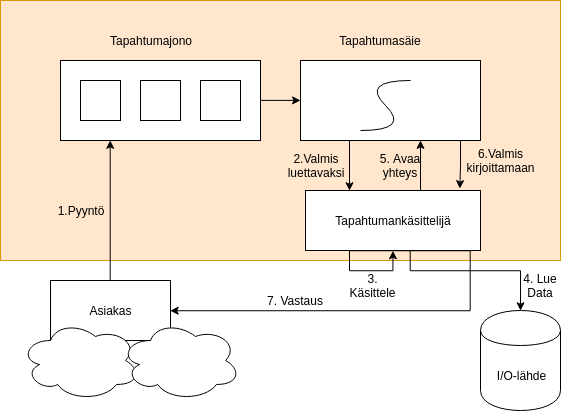
\includegraphics[scale=0.6]{reactor.png}\label{fig:reactor}
\end{figure}

Mallin tapahtumakäsittelijöissä samanaikaisuuteen päästään
vain I/O:n osalta, kun käytetään asynkronisia
I/O-operaatiota.
Estäviä operaatioita tulee välttää,
sillä niiden käyttäminen laskee sovelluksen
tehokkuutta huomattavasti~\cite{schmidt_reactor:_1995}.
Asynkronisia I/O-operaatioita
voidaan suorittaa niitä tarjoavien käyttöjärjestelmäkutsujen
avulla, tai siirtämällä I/O-operaatiot toisen säikeen tehtäväksi.
Itse Reactor-malli ei ota kantaa siihen, miten asynkroninen operaatio toteutetaan.
Jos tapahtumakäsittelijässä tarvitaan pitkäkestoista laskentaa,
kannattaa sitä varten luoda uusi prosessi tai säie. Tämä
prosessi tai säie saattaa pyynnön loppuun rinnakkain
tapahtumasäikeen kanssa~\cite{schmidt_reactor:_1995}.

Reactor-toteutuksissa tapahtumiksi mallinnetaan I/O-väylien
valmiutta suorittaa luku-tai kirjoitusoperaatioita~\cite{schmidt_reactor:_1995}.
Kun I/O-väylä
vapautuu, tapahtumasäie viestii tapahtumakäsittelijälle, että 
I/O-operaation voi suorittaa. Sovellus siis toisin sanoen
reagoi I/O-laitteen vapautumiseen ja tästä nimi Reactor juontuu.
Näin käyttöjärjestelmä ei aseta
verkkopalvelinsovellusta odottaa tilaan I/O-operaatioiden takia.
Reactor-mallin palvelintoteutuksista käytetään kirjallisuudessa
usein nimeä SPED(Single Process Event Driven).


\subsection{Proactor}

Reactor-malli on osa Proactor-mallia.
Siinä hyödynnetään käyttöjärjestelmän asynkronisia ominaisuuksia suorittamaan
operaatiota ennen pyynnön saapumista tapahtumasäikeelle~\cite{hu_applying_1998}.
Reactor-mallinen osa ohjaa tässä mallissa asynkronisten tapahtumien
valmistumistapahtumia niitä vastaaville tapahtumankäsittelijöille~\cite{pyarali_proactor_1997}.

Toisin kuin Reactor-mallinen palvelin, joka reagoi I/O-laitteen vapautumiseen,
Proactor-mallinen palvelin~\cite{hu_applying_1998} reagoi vasta kun, käyttöjärjestelmä
on suorittanut I/O:n asynkronisesti sen puolesta. Tästä käytetään nimitystä
proaktiivinen I/O semantiikka~\cite{schmidt_reactor:_1995}.

Proactor mallin tavoite on yksinkertaistaa asynkronisten ohjelmien kehitystä.
Proactor-mallissa voidaan suoraviivaisesti suorittaa toisistaan riippuvaisia
asynkronisia operaatioita, asettamalla asynkronisten tapahtumien valmistumisille
käsittelijöitä. Eli toisin sanottuna asynkronisten operaatioiden vastakutsuista
voi kutsua uusia vastakutsuja. Näin voidaan rakentaa riippuvaisten
asynkronisten operaatioiden ketjuja. Ketjuilla voidaan
rakentaa peräkkäistä I/O-logiikkaa estämättä muiden asiakkaiden
pyyntöjen käsittelyä.

Proactor-mallia suositellaan käytettäväksi, jos sovellus vaatii
asynkronisten operaatioiden kutsumista ja sovellus tarvitsee ilmoituksen
asynkronisen operaation valmistumisesta~\cite{pyarali_proactor_1997}.
Pyyntöjen käsittely Proactor-mallissa käydään läpi kuvassa~\ref{fig:proactor}.
Kuva~\ref{fig:proactor} noudattaa Proactorin~\cite{hu_applying_1998} esittelyyn tehtyä
kuvaa, jossa Proactor-palvelin käsittelee pyynnön, mutta kuvassa~\ref{fig:proactor}
korostetaan Proactoriin-sisältyvää Reactor-mallia.
\begin{figure}
  \caption{Pyynnön käsittely Proactor-mallissa. Mukautettu lähteestä~\cite{hu_applying_1998}}
  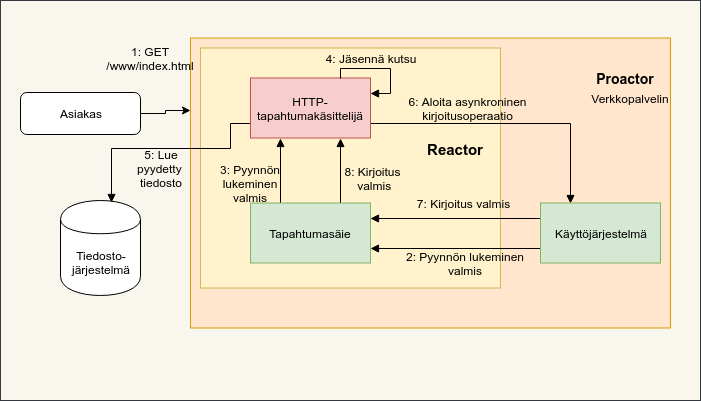
\includegraphics[scale=0.6]{Proactor.png}\label{fig:proactor}
\end{figure}
Pyynnön käsittely Proactor-mallisessa palvelimessa~\cite{hu_applying_1998} 
tapahtuu seuraavasti:
    \begin{enumerate}
      \item Asiakas lähettää HTTP GET pyynnön.
      \item Käyttöjärjestelmä lukee pyyntöä sovittuun puskuriin ja ilmoittaa kun valmis.
      \item Valmistumisohjaaja (Reactor) kutsuu HTTP-tapahtumakäsittelijää.
        Kohdat 2 ja 3 toistuu kunnes koko pyyntö on luettu.
      \item HTTP-tapahtumakäsittelijä jäsentää kutsun. Eli
        käytännössä selvittää minkä tiedoston asiakas haluaa.
      \item HTTP-tapahtumakäsittelijä lukee pyydetyn tiedoston.
      \item HTTP-tapahtumankäsittelijä aloittaa asynkronisen operaation
        kirjoittaakseen tiedoston datan asiakasyhteyteen, ja asettaa
        itsensä tapahtumakäsittelijäksi kirjoituksen valmistumiselle.
      \item Kun kirjoitusoperaatio on valmis käyttöjärjestelmä ilmoittaa
        Valmistumisohjaajalle.
      \item Valmistumisohjaaja huomauttaa HTTP-tapahtumakäsittelijää,
        koska se asetti itsensä tapahtumankäsittelijäksi kirjoituksen
        valmistumiselle. Kohtia 6 - 8 toistetaan kunnes koko tiedosto on lähetetty.
    \end{enumerate}
Reactor-mallin tavoin Proactor-malli ei myöskään sovellu laskennan rinnakkaistamiseen.
Proactor-mallin muutokset Reactor-malliin rajoittuvat
asynkronisten-operaatioden ohjaamisen
kehittämiseen. Mallissa tapahtumasäie kutsuu tapahtumankäsittelijöitä, jolloin
pitkäkestoisen laskennan suorittaminen tapahtumankäsittelijässä, johtaisi
muiden pyyntöjen odotusajan kasvuun. Malliin pitää siis
lisätä muita mekanismeja laskennan suorittamiseen rinnakkain.

Moniprosessorikoneella Proactor-mallin toteutukseen
ehdotetaan~\cite{pyarali_proactor_1997}, että valmistumistapahtumia suorittaisi
säiereservitoteutus
eikä Reactor-toteutus. Näin laitteiston useita suorittimia voisi hyödyntää.

Modernissa verkkopalvelinsovelluksessa Proactor-mallin suosioon on
monta syytä. RESTful-rajapinnan käyttäminen
verkkopalvelinsovelluksessa viestien välitykseen,
saa yksittäisten viestien koon pysymään pienenä ja viestien
käsittelyyn kuluvan ajan lyhyempänä verrattuna
HTML-tiedosto vastaukseen, sillä
vastaukseen liittyy vain halutun dataresurssin tietoja.
Rinnakkaisuus
voidaan järjestelmän arkkitehtuurissa siirtää tietokantamoottorin vastuulle,
jolloin verkkopalvelin voi lähettää sille asynkronisia kyselyitä
ja näin suorittaa useisiin pyyntöihin liittyviä tietokantakyselyitä
samanaikaisesti. Tämä vaatii Proactor-mallin sillä, asynkronisen tietokantaoperaatioon
pitää kytkeä vastakutsu tiedon käsittelyyn ja lähettämiseen.
Tämänkaltaisella toteutuksella verkkopalvelimen käyttötapaus sopii
hyvin yhteen Proactor-mallin määrittelyn kanssa tukeutuen
mallin vahvuuksiin sekä peittäen sen heikkouksia.

\subsection{AMPED}

AMPED on asynkroninen tapahtumaohjattu malli, jossa
tapahtumasäie suorittaa suurimman osan prosessoinnista. 
Sen erikoispiirre on, että estävät I/O-kutsut
siirretään apulaisten vastuulle, jolloin
ne ei estä tapahtumasäiettä~\cite{pai_flash_1999}. Apulaiset voivat
olla joko prosesseja tai ydintasonsäikeitä.
AMPED-malli siis sisältää säiereservimallin.
Tällä mekanismilla muutetaan käyttöjärjestelmän
estävät pyynnöt tapahtumasäikeen näkökulmasta
asynkronisiksi.
AMPED-mallin tavoite~\cite{pai_flash_1999} on säilyttää Reactor-mallin
edut järjestelmissä, joissa asynkronisten
kutsujen tuki on huono.

Nykyään suosittu tapahtumaohjatun palvelimen toteutus on
käyttää Node.js sovellusympäristöä. Node.js ympäristössä
on vaikutteita Proactor-ja AMPED-malleista.
Node.js:n tapahtumaohjatun mallin toteuttamisesta vastaa
libuv-kirjasto~\cite{libuv_design_2019}. Suunnittelufilosofiassa
libuv:lla on paljon yhteistä AMPED-mallin kanssa, sillä
sen tarkoitus on taata aina asynkroniset I/O-operaatiot alustasta
riippumatta. Libuv siirtääkin I/O-kutsun toiselle säikeelle
jos alustalla ei ole tarjota asynkronista kutsua~\cite{libuv_design_2019}.
Tämä toimintapa saa kutsun näyttämään tapahtumankäsittelijästä
asynkroniselta. Libuv myös tarjoaa myös mahdollisuuden
käsitellä asynkronisten operaatioiden valmistumisia, kuten 
Proactor-malli tekee.

\subsection{SEDA ja SYMPED}

Toinen Reactor mallin laajennus on SEDA (Staged Event Driven Architecture)~\cite{welsh_seda_2001}.
SEDA-mallin tavoitteisiin kuuluu samanaikaisuus suuressa mittakaavassa ja
verkkopalveluiden kehittämisen yksinkertaistaminen.
SEDA-mallinen sovellus voi itse analysoida omaa toimintaansa
ja säätää käyttämiään resursseja sen  mukaan.
Se käyttää tapahtumaohjattuja menetelmiä niiden soveltuessa, mutta
kykenee käyttämään säikeitä tarvittaessa.

Siinä pyyntöjen käsittely jaetaan tasoiksi, joissa kaikissa on
käytännössä Reactor-mallin toteuttava rakenne. Jokaisella tasolla
on oma tapahtumajono sekä tapahtumakäsittelijä, joka ohjaa työtä
apusäikeille. Tasoilla ei ole tapahtumasäiettä, sillä
jokaisella tasolla on vain yksi tapahtumakäsittelijä.
Tapahtumakäsittelijä voi käsittelyn päätteeksi
lisätä uusia tapahtumia seuraavien tasojen tapahtumajonoihin.
Tämän lisäksi jokaisella tasolla on resurssiohjaaja,
joka vastaa resurssien käytön pysymisestä sallitulla tasolla,
sekä apusäikeiden määrästä kyseisellä tasolla~\cite{welsh_seda_2001}.
SEDA-mallissa sovellus koostuu tasojen verkosta, jotka
yhdistetään tapahtumajonoilla.
SEDA-mallin suurin ero Reactor-malliin
on sen hienojakoisempi resurssien ohjaus 
tapahtumankäsittelyn eri tasoille.
SEDA-arkkitehtuurilla on mahdollista myös saavuttaa rinnakkaisuutta
laskennallisesti vaativissa tehtävissä~\cite{welsh_seda_2001}. Laskennallisesti
vaativalle ja rinnakkaiselle tehtävälle tapahtumankäsittelyssä voidaan
luoda taso, jolla on suuri säiereservi.

Hadoob~\cite{welsh_seda_2001} verkkopalvelinsovellus on toteutettu SEDA-mallin mukaisesti.
Siinä verkkoyhteyksien kuuntelulle on oma taso, jonka tehtävä
on hyväksyä yhteys. Yhteyden hyväksymisen jälkeen taso siirtää yhteyden
HTTP-pyynnön jäsentämistasolle, jolla pyyntö jäsennetään ja siirretään
sivuvälimuistin tarkastavaan tasoon. Jos pyydetty sivu löytyy välimuistista,
siirretään välimuistista löytynyt sivu HTTP-pyynnön lähettämistasolle, jossa
tarvittavat kehystiedot lisätään viestiin. Lopulta
viesti siirretään verkkoyhteyteen kirjoittavalle tasolle, joka
kirjoittaa vastauksen asiakkaalle.

Reactor-mallia voi laajentaa vielä kolmannella tavalla.
Jos samaa Reactor-sovellusta ajaa yhdessä eri säikeillä tai prosesseilla
ja jokin säie jakaa työn tasaisesti tapahtumasäikeiden välillä
on kyseessä SYMPED-malli. Näin Reactor-toteutuksen
skaalautuvuutta voidaan jälkikäteen parantaa.
SYMPED-mallissa yhdistetään siis Reactor-malli säie-tai prosessireserviin.
SYMPED ja AMPED mallien ero on siinä, että 
AMPED-mallissa säikeitä käytetetään vain apulaisina
estävien operaatioiden suorittamiseen, kun taas
SYMPED-mallissa jokaisella säikeellä on oma palvelimensa,
joka suorittaa sille jaettujen pyyntöjen käsittelyn
kokonaisuudessaan.


\section{Mallien vertailu ja analyysi}\label{sec:vertailu}
% TODO: Lisää esimerkkejä mallien analyysiin
Tässä luvussa vertaillaan ja analysoidaan
suunnittelumallien toteutuksia.
Vertailu perustuu kirjallisuudessa
tehtyihin testeihin ja arvioihin
mallien soveltuvuudesta eri
käyttötapauksiin.
Vertailua ohjaava ajatus on:
edistääkö mallin käyttäminen palvelimen
suorituskykyä 
nostamatta sovelluslogiikan kehitystyön haastavuutta
sietämättömälle tasolle.
Seuraavaksi esitellään arviointikriteerit,
joilla malleja vertaillaan.
\subsection{Arviontikriteerit}
% TODO: Kriteereille lähteet


Järjestelmien vertailuun on valittu seuraavat kriteerit:
\begin{itemize}
  \item suorituskyky
    \begin{itemize}
      \item käsiteltyjen pyyntöjen määrä eli volyymi
      \item skaalautuvuus laitteistoresursseihin
      \item viive
    \end{itemize}
  \item vakaus
  \item kehitystyön haastavuus
\end{itemize}


Palvelimen roolin kannalta olisi toivottavaa, että
se pystyisi käsittelemään mahdollisimman paljon pyyntöjä
tietyssä ajassa.
Suorituskykyinen palvelin on edullinen
palvelun ylläpitäjälle~\cite{pai_flash_1999}.
Pyyntöjen volyymia voidaan
mitata täytettyjen pyyntöjen määrällä ajan suhteen.

Yksittäiselle asiakkaalle tärkein suorituskyvyn mittari on se, kuinka kauan
yksittäiseen pyyntöön vastaaminen vie.
Pyynnön pieni viive saa
palvelun käyttökokemuksen tuntumaan sujuvammalta.
Viivettä mitataan millisekunteina.
Pyyntöjen keskimääräinen viive ja käsiteltyjen pyyntöjen
volyymi ovat kääntäen verrannollisia, koska
mitä nopeammin yksittäisen pyynnön voi käsitellä sitä
enemmän pyyntöjä voidaan palvella aikavälillä.

Skaalautuvuus on tärkeää palvelinta ylläpitävälle taholle, sillä
näin käyttäjämäärän kasvaessa voidaan suorituskykyä parantaa
lisäämällä laitteistoresursseja. Skaalautuvuutta voidaan
mitata testaamalla mallien toteutuksia eri tehoisilla laitteistoilla
ja vertailemalla, kuinka paljon suorituskyky muuttuu 
parantuneiden laitteistoresurssien myötä.

Verkkopalvelinsovelluksen tulisi
olla vakaa. Vakauden määrittää
se todennäköisyys, joka sovelluksella on
päätyä kriittiseen virhetilanteeseen. Kriittisessä
virhetilanteessa sovellus ei osaa
itse palautua sellaiseen tilaan, jossa
toiminta voisi jatkua normaalisti ja oikein.
Virhetilaan voidaan päätyä käytännössä
ohjelmointivirheen, laitteistovirheen tai hyökkäyksen seurauksena.
Verkkopalvelinsovelluksen suunnittelumalli
vaikuttaa etenkin ohjelmointivirheiden todennäköisyyteen
ja voi tehdä tietyistä hyökkäyksistä lamauttavampia.


Verkkopalvelimen suunnittelumallin tulisi
yksinkertaistaa samanaikaisuuden hallintaa sovelluksessa~\cite{hu_applying_1998}.
Kehitystyön helpottaminen vähentää kustannuksia,
kun järjestelmää rakennetaan, laajennetaan ja ylläpidetään.
Siksi järjestelmän rakenteen yksinkertaisuus ja
ymmärrettävyys on haluttava ominaisuus.

\subsection{Toteutusten suorituskyky}
Vuonna 1997 James C. Hu et.al~\cite{hu_measuring_1997} testeissään huomasivat,
että pienillä tiedostoilla säiereservimallia noudattava palvelintoteutus oli paras,
mutta suuremmilla tiedostoilla Proactor-toteutus oli kaikista tehokkain.
Testissä Proactor-toteutuksen asynkronisia operaatioita hidasti
erityisesti TransmitFile-funktio, joka oli
hidas pienillä tiedostoilla.
Proactor-toteutus käytti tätä kutsua I/O:n hallitsemiseen,
kun taas säiereservi-toteutus käytti estävää I/O:ta.

Tästä tuloksesta voidaan huomata,
että suurilla tiedostoilla asynkroniset kutsut
pitävät I/O-resurssien käyttöasteen hyvin suurena.
Käyttöjärjestelmä pystyy siis tehokkaasti aikatauluttamaan
I/O-laitteilla suuria asynkronisia operaatioita.

TransmitFile-funktio aiheutti pienillä 500-tavuisilla tiedostoilla hyvin suuren viiveen
vastauksille. Viive oli noin 200 ms. Samalla tiedostokoolla säiereservimallin toteutus
suoriutui vain noin 50 ms viiveellä.
50:n kilotavun kokoisilla tiedostoilla Proactor-toteutuksen
viive laski alle säiereservimallin arvon.
Myös tätä suuremmilla tiedostoilla Proactor-toteutus oli säiereservimallin toteutusta nopeampi.
Pienillä tiedostoilla säireservimallin toteutuksella oli suurempi
volyymi, mutta suurilla tiedostoilla Proactor-toteutus
kykeni suurempaan volyymiin.

Pohdittavaksi jää miten uudemmat käyttöjärjestelmissä
toteutetut asynkroniset kutsut suoriutuisivat 
vastaavassa kokeessa.

Ivan Voras ja Mario Zagar testasivat~\cite{voras_characteristics_2009},
palvelimen suunnittelumalleja mdcached keskusmuistitietokantaan.
Testissä oli mukana Reactor-toteutus, SEDA-toteutus ja AMPED-toteutus.
Keskusmuistitietokannan erikoispiirre on, että siihen ei liity lainkaan levy I/O:ta.
Siten toteutuksen suorituskyky on pääasiassa riippuvainen muistiväylän nopeudesta sekä
käyttöjärjestelmäkutsujen nopeudesta. Tämä eroaa tavanomaisesta
verkkopalvelinsovelluksesta, jossa usein tarvitaan levy-I/O:ta 
eri tiedostojen lukemiseen.
Mallien toteutuksista mitattiin operaatioiden (transaction) määrä sekunnissa vaihtuvilla tietyillä
asiakasmäärillä. Kaikki mallit testattiin samalla laitteistolla.


Testissä selvisi että, heidän SEDA-toteutuksensa kahdella tapahtumasäikeellä ja neljällä apusäikeellä
ei saavuttanut huomattavaa
etua Reactor-toteutukseen~\cite{voras_characteristics_2009}. Tämän diagnosoitiin
johtuvan SEDA:n aiheuttamien suoritinympäristön vaihtojen yleisyydestä
sekä säikeiden välisestä kommunikoinnista.
Testissä molempien toteutuksien suorituskyky
oli lähes samalla tasolla 120:een asiakkaaseen asti, jota
suuremmilla asiakasmäärillä Reactor-toteutuksen suorituskyky alkoi
hieman heikentyä.Reactor-toteutus suoritti silloin noin 110 000 toimitusta sekunnissa
ja SEDA-toteutus 120 000 sekunnissa.

SEDA-mallissa jokaisella käsittelyn vaiheella on omat apusäikeensä,
joilla saadaan rinnakkaistettua vaiheeseen liittyvää estävää laskentaa.
Muistitietokannan käyttötapauksessa estävää laskentaa on vähäisesti.
Kuitenkin vaiheesta toiseen siirtyminen aiheuttaa suoritinympäristön vaihdon,
kun uuden vaiheen apusäie otetaan käyttöön.
Apusäikeiden hyödyt
tulisivat näkyviin selkeämmin käyttötapauksessa, jossa vaaditaan enemmän
rinnakkaista estävää laskentaa kuin muistitietokannan tapauksessa.

Samassa testissä~\cite{voras_characteristics_2009} AMPED-toteutus neljällä apuprosessilla
kykeni 250 000 toimitukseen sekunnissa 120:llä asiakkaalla. Mielenkiintoista on,
että heidän SEDA-toteutus, jossa tapahtumasäikeiden ja apusäikeiden
määrät asetettiin samaksi, suoriutui huomattavasti paremmin ja
saavutti 300 000 tapahtumaa sekunnissa 120:llä asiakkaalla.
Vertailun selkein voittaja skaalautuvuuden
osalla oli SYMPED-toteutus.
Tällä toteutuksella neljällä säikeellä
saavutettiin 440 000 toimitusta sekunnissa 120:llä asiakkaalla.
SYMPED-toteutus osoitti myös hyvää skaalautuvuutta
sille annettujen säikeiden määrän kasvaessa.
Koska muistitietokannan toiminta eroaa
hyvin paljon verkkopalvelimesta, ei näitä
tuloksia voi suoraan käyttää verkkopalvelinsovelluksien 
vertailuun.

Harji et.al testasivat~\cite{harji_comparing_2012} suunnittelumalleja 
modernilla neliytimisellä moniprosessoritietokoneella. Tutkimuksessa
testattiin SYMPED-ja SEDA-malleja sovellettuina verkkopalvelinsovellukseen.
Niistä testattiin toteutukset pohjautuen prosesseihin ja
ydintasonsäikeisiin.
Vertailukohtana oli myös avoimen lähdekoodin palvelimia kuten Apache. Apachen 
versio 2.2.9 on toteutettu säie-yhteyttä-kohti mallilla, jossa
jokaista pyyntöä kohti luodaan uusi säie, ja vastauksen jälkeen säie tuhotaan.
Testauksessa asiakkaat käyttävät httperf-testausohjelmaa lähettääkseen
sarjan pyyntöjä palvelimille.
Testejä suoritettiin kaksi, ensimäisessä palvelimen muistimäärä
oli rajoitettu neljään gigatavuun ja toisessa kahteen.

Testien tuloksista huomataan, että SYMPED-ja SEDA-mallit
ovat hyvin suorituskykyisiä moniprossesorikoneella riippumatta käytetäänkö
toteutuksissa säikeitä vai prosesseja. Testeissä ne pystyivät
neljän gigabitin testin aikana välittämään jopa noin 6000 megabittiä sekunissa,
kun taas Apache-palvelimen nopeus jäi vain hieman yli 2000:n megabittiin
sekunissa.

Apachen huonon suorituskyvyn~\cite{harji_comparing_2012} 
todetaan johtuvan säie-yhteyttä-kohti mallin
ominaisesta säikeiden hallinnointiin kuluvasta laskentatehosta.
ydintasonsäikeitä syntyy yksinkertaisesti niin paljon,
ettei niiden hallinnointiin kuluvaa aikaa saa 
takaisin rinnakkaisuuden antamalla edulla.

SYMPED- ja SEDA-toteutuksien todetaan olevan vain 10 $\%$ päässä
toisistaan~\cite{harji_comparing_2012}. Se käytettiinkö toteutuksessa
prosesseja vai säikeitä
näkyy lähinnä muistijalanjäljessä, jossa säikeillä toteutettu versio
pärjää vähemmällä muistilla, sillä säikeet jakavat
yhteisen muistialueen. Prosessitoteutuksella muistiin tulee
samaa tietoa useita kertoja.

\subsection{Sovelluslogiikan kehitystyön haastavuus}
Verkkopalvelinsovelluksen suunnittelumalli on työkalu kehittäjälle,
joka toteutetaan mielekkäästi kirjastona tai moduulina.
Jos malli on hyvin toteutettu, kehittäjän tulisi pystyä
keskittymään keskeisen sovelluslogiikan kirjoittamiseen
murehtimatta rinnakkaisuutta hallitsevasta osasta.

Reactor-malli on yksinkertainen ja helpommin toteutettava
kuin Proactor. Reactor-malli onnistuu hyvin tavoitteessaan
erottaa pyyntöjen samanaikaistamiseen liittyvä logiikka
muusta sovelluslogiikasta.
Tapahtumaohjatut sovellukset tuovat omat haasteensa
kehittäjälle, sillä niistä virheiden löytäminen ja
korjaaminen on usein työlästä, koska ohjelman
suoritus ei kulje rivi riviltä, vaan järjestys
muuttuu tapahtumakäsittelijöiden ja vastakutsujen mukaan.

Reactor-mallia käyttävässä palvelimessa kehittäjän
pitää huolehtia siitä, että yksittäisen pyynnön
käsittelyyn menee vähän aikaa~\cite{schmidt_reactor:_1995}, koska
tapahtumasäikeen aika pitää jakaa tehokkaasti
kaikkien pyyntöjen välillä. Tämä saavutetaan
vähentämällä viesteihin liittyvää laskentaa optimoimalla ja
asynkronisilla I/O-kutsuilla.

Reactor-mallin toteutuksissa kehittäjän tulee huomioida
asynkronisen I/O:n vaikutukset. Asynkronisuus vaikeuttaa koodin
luettavuutta, mutta se nostaa ohjelman samanaikaisuutta ja täten
tehokkuutta huomattavasti. Sovelluslogiikan kehittäjän
tulee huolehtia, että kirjoitettava logiikka
käyttää asynkronisia kutsuja~\cite{schmidt_reactor:_1995}, sillä estävät
kutsut pysäyttävät koko sovelluksen suorituksen.

Ongelmana on myös pidetty käyttöjärjestelmien huonoa
tukea asynkronisille kutsuille~\cite{pyarali_proactor_1997}. Järjestelmäkutsu
$select$, johon perustui käyttöjärjestelmien Reactor-toteutuksia,
ei salli useamman säikeen odottaa saman tunnistejoukon tapahtumia.
Tämä ominaisuus estää tehokkaan laitteiston rinnakkaisuuden hyödyntämisen.
Asynkronisten kutsujen tuki on kuitenkin parantunut.
Linux-ytimen versiossa
2.4.44 siihen lisättiin $epoll$~\cite{man_epoll} järjestelmäkutsu, joka
sallii tapahtumapohjaisen I/O:n useammalla säikeellä

samaan aikaan.
Jos ohjelman tulee käsitellä
asynkronisen operaation tulosta, tulee operaation valmistumiselle
asettaa vastakutsu. 
Tässä tilanteessa Proactor-malli on erittäin hyödyllinen, sillä se
kuvailee selkeästi miten asynkronisten tapahtumien valmistumisia tulisi käsitellä.

Proactor-mallissa kuten Reactor-mallissa sovelluslogiikka ohjelmoidaan
tapahtumankäsittelijöihin, mutta Proactor-mallissa logiikkaan liittyy
tyypillisesti vastakutsuja 
asynkronisten operaatioiden valmistumisille. Jos 
niille ei tarvita vastakutsuja,
voidaan vain käyttää Reactor-mallia ilman Proactor-rakennetta.
Vastakutsujen ketjutus on tehokas työkalu hallitusti käytettynä,
mutta liikaa käytettynä se tekee ohjelman kulusta vaikeasti
hahmotettavan.

Reactor-tai Proactor-mallit eivät tarjoa keinoja
suorittaa laskentaa rinnakkain. Kehittäjän tulee lisätä
mallin tapahtumakäsittelijöihin rinnakkaisuutta käsittelevää
logiikkaa kuten säikeiden luomista, silloin kun se on tarpeen.

Säiereservimallissa ohjelmakoodi voidaan pitää yksinkertaisena ja
hyvin luettavana. Kehittäjät voivat vapaasti käyttää intuitiivisia
peräkkäisiä operaatioita ja estäviä kutsuja, koska sovelluslogiikkaa
suoritetaan erillisillä säikeillä~\cite{hu_applying_1998}. Estävä kutsu pysäyttää vain
sen säikeen, jonka käsittelyyn se liittyy, jolloin muiden
pyyntöjen käsittely voi jatkua esteettä.

Eri asiakkaiden pyynnöt liittyvät harvoin toisiinsa,
jolloin niiden välillä ei ole merkittävästi jaettua tilatietoa ja
synkronointia tarvitaan minimaalisesti.
Kehittäjän tulee kuitenkin ottaa huomioon mahdolliset lukkiutumiset
ja kilpailutilanteet eri pyyntöjen välillä, jos
toteutuksessa ilmenee tarve tilatiedon tai resurssien jakamiselle.
Pyyntöihin liittyvä laskenta rinnakkaistuu hyvin laitteistotasolla,
kun jokainen pyyntö on käsittelyssä omalla säikeellään.

SEDA-mallissa rinnakkaisuuden hallintaa edistää
samaa tietoa käsittelevien säikeiden eristäminen samalle tasolle~\cite{welsh_seda_2001}.
Samalla tasolla synkronisoiminen ja kilpailutilanteiden ratkaiseminen on
yksinkertaisempaa kuin koko sovelluksen mittakaavassa, ja
viesteihin perustuva sovelluksen kulku on helpommin seurattavissa kuin
muissa tapahtumaohjatuissa malleissa.

Jos Reactor-palvelimen skaalautuvuus ei riitä palvelemaan
järjestelmän tarpeita, voidaan järjestelmän sovelluslogiikka
sovittaa suoraviivaisesti osaksi SYMPED-toteutusta. SYMPED-toteutus
voidaan rakentaa reactor eli SPED toteutuksen ympärille. Tämä
tekee SYMPED-toteutuksesta mielekkään jatkosuunnitelman kehittäjälle,
jonka huolet skaalautuvuudesta koskevat pääasiassa palvelun tulevaisuutta.
Järjestelmään pitää vain siis lisätä rakenne, joka
jakaa työt eri prosesseilla ajettavien Reactor-palvelimien välillä.
Tämän lisäksi tulee varmistua siitä, että tapahtumakäsittelijöiden
logiikka ei aiheuta lukkiutumisia eri prosessien välillä.

\subsection{Vakaus}
Palvelimen vakaudella tarkoitetaan sen kykyä vastustaa hyökkäyksiä ja
virhetiloja.
Palvelimen suunnittelumalli vaikuttaa sen vakauteen, jos asiakkaiden
pyynnöt vaikuttavat toisiinsa tai jos rinnakkaistaminen voi aiheuttaa virhetiloja kuten
lukkiutumista.

Reactor/Proactor-malliseen palvelimeen voi kohdistaa hyökkäyksiä, joilla pyritään
myrkyttämään sovelluksen tapahtumasäie~\cite{davis_case_2017}. Reactor-mallin palvelintoteutuksissa
osoitepolkujen jäsentäminen on saman säikeen vastuulla kuin sovelluksen ohjaaminen.
Tämän työvaiheen takia
tapahtumasäikeen myrkyttämiseen sopivat pyynnöt,
joiden osoitepolun selvittämiseen liittyy kompleksista
säännöllisten lauseiden käsittelyä~\cite{davis_case_2017}.
Proactor-mallin kuvassa~\ref{fig:proactor} pysähdyttäisiin 
siis kohtaan 4: kutsun jäsentäminen, ja
kaikki muut pyynnöt joutuvat odottamaan.
Yksi pyyntö siis aiheuttaa suhteettoman suuren työtaakan
tapahtumasäikeelle, jolloin koko sovellus jää odottamaan sitä.
Hyökkääjä lähettää näitä pyyntöjä niin paljon, että sovellus
ei pysty palvelemaan sen todellisia asiakkaita. Tämä
on hyökkäys kuuluu palvelunestohyökkäyksiin.

Tällaiset hyökkäykset aiheuttaisivat ongelmia myös säiereservimallia
noudattaville järjestelmille, mutta niiden pitäisi onnistua
myrkyttämään reservin jokainen säie samaan aikaan, jotta
järjestelmä ei kykenisi enää vastaamaan asiakkaiden pyyntöihin~\cite{davis_case_2017}.

Yhdellä säikeellä toteutetulla tapahtumaohjatulla palvelinsovelluksella ei ole
riskiä sisäisille kilpailutilanteille tai lukkiutumiselle, koska
yksi säie ei voi ajautua kilpailemaan itsensä kanssa resursseista.
Säiereservimallissa palvelin voi lukkiutua, jos samaan aikaan käsittelyssä olevat
pyynnöt tarvitsevat samoja resursseja käsittelyn aikana. Tämä riski on otettava
huomioon järjestelmän suunnittelussa ja sovelluslogiikan kirjoittamisessa.

Säiereservimallissa kilpailutilanteiden riski on hyvin pieni, jos pyyntöjen
välillä ei ole jaettua tilatietoa. Jaetun tilatiedon kanssa voi tulla
sivuvaikutuksia, jos pyynnöillä on mahdollisuus muokata tilatiedon sisältöä.
SEDA-mallissa kilpailutilanteiden hallintaa helpottaa synkronoinnin
rajaaminen yhdelle tasolle~\cite{welsh_seda_2001}.

\subsection{Johtopäätökset}
Reactor-malli~\cite{schmidt_reactor:_1995} erottaa
selkeästi pyyntöjen käsittelyn
samanaikaistamiseen liittyvän
logiikan muusta sovelluskohtaisesta logiikasta.
Malli on yksinkertainen verrattuna muihin samanaikaisuutta
käsitteleviin malleihin.
Näistä syistä se on toteutettu useisiin
kirjastoihin ja saavuttanut vakaan suosion.

Reactor-mallin kyvyttömyys suorittaa rinnakkaista laskentaa 
ei ole haitaksi, jos järjestelmässä on rinnakkaisuutta
korkeammalla tasolla~\cite{schmidt_reactor:_1995}. Eli
Reactor-mallisia palvelimia ajetaan useita rinnakkain
ja näin luodaan SYMPED-järjestelmä.

Proactor-malli laajentaa Reactor-mallia merkittävällä tavalla
kehitystyön näkökulmasta,
sillä sen avulla voidaan ketjuttaa asynkronisia
operaatioita luontevasti vastakutsuilla. Tämä ominaisuus
tuo joustavuutta samanaikaisen sovelluslogiikan kehittämiseen.

Proactor-mallin ansiosta rinnakkaisuus
voidaan toteuttaa myös 
muualla palvelun kokonaisuudessa kuten tietokantaohjelmassa.
Proactor-palvelin voi odottaa useita asynkronisia
tietokantakyselyita samalla, kun se suorittaa
muuta logiikkaa. Eli tietokantakyselyn valmistumiskäsittelijäksi
asetetaan toiminto, joka kirjoittaa vastauksen
halutussa muodossa asiakkaalle.
Todellisen rinnakkaisen työn
suorittaa tässä tapauksessa tietokantaohjelma.

Proactor-malli ei paikkaa
Reactor-mallin rajallisuutta laskennan rinnakkaisuudessa~\cite{pyarali_proactor_1997},
sillä tapahtumakäsittelijöiden logiikka suoritetaan
samalla säikeellä kuin sovelluksen kulun ohjaus.
Laskennan rinnakkaistamiseksi tapahtumakäsittelijöihin
tulee lisätä säikeiden käsittelyyn liittyvää logiikkaa
tai vaihtaa valmistumistapahtumien käsittelystä vastaava
osa Reactor-toteutuksesta säiereservitoteutukseen.
Malli ei siis vähennä laskennan rinnakkaisuuteen liittyviä
haasteita, mutta on tehokas tapahtumien ja asynkronisten
operaatioiden hallinnassa~\cite{hu_applying_1998}.
Nämä ominaisuudet riittävät
I/O-resurssien tehokkaaseen hyödyntämiseen.

Reactor/Proactor-mallin toteuttavalla
kirjastolla voidaan kustannustehokkaasti
toteuttaa palvelin, joka kykenee suoriutumaan
tehtävistään palvelun alkutaipaleella. Jos
käyttäjämäärät kasvavat ja skaalautuvuutta
vaaditaan voidaan järjestelmä muuttaa SYMPED-järjestelmäksi,
joka skaalautuu hyvin resursseihin.
Node.js sovelluksesta voi luoda SYMPED järjestelmän
cluster-moduulilla~\cite{noauthor_cluster_nodate}.
Cluster-moduulilla on helppo luoda useita lapsiprosesseja,
jotka jakavat verkkopalvelinsovellukselle määritetyt
portit. Moduuliin sisältyy rakenne,
joka oletuksena jakaa työn lapsiprosessien välillä
round-robin-menetelmällä.

Jos laskennan suorittaminen rinnakkain usealla suorittimella
on ainoa väylä riittävän suorituskyvyn saavuttamiseksi,
ovat säiereservimalli, SYMPED ja SEDA-malli hyviä vaihtoehtoja.
SEDA-mallissa rinnakkaisuus on selkeästi rajoitettu
pyynnön käsittelyn tietylle tasolle.
SYMPED-mallissa pyyntöjä suoritetaan rinnakkain
ja yksittäiset säikeet hyödyntävät
tapahtumaohjattua ohjelmointia.
\section{Yhteenveto}\label{sec:yhteenveto}

Verkkopalvelimen voi esittää luontevasti
tapahtumaohjattuna mallina. Reactor-malli esittää yksinkertaisen
ratkaisun useista lähteistä tulevien tapahtumien käsittelyyn 
ja sopii tapahtumaohjatun palvelimen rakentamiseen.

Verkkopalvelimen yleisimmät tehtävät ovat
HTML-tiedostojen ja nykyään kasvavissa määrin
muun tekstimuotoisen datan lähettäminen.
Näiden tehtävien suorituskyky on
I/O-sidonnainen.
Asynkronisilla luku-ja kirjoitusoperaatioilla samanaikaisen I/O:n hallinta
voidaan siirtää käyttöjärjestelmän vastuulle, joten Proactor-mallinen palvelin
sopii hyvin
verkkopalvelimen tehtävien täyttämiseen.
Se esittää sopivat laajennukset Reactor-malliin, joilla
asynkronisia operaatioita voidaan hallita joustavasti.
Sillä voidaan suorittaa muista asynkronisista operaatioista riippuvaisia I/O-operaatioita
samanaikaisesti, ketjuttamalla niitä vastakutsuilla.
Asynkronisilla operaatioilla voidaan saavuttaa suuri I/O-resurssien
käyttöaste.

Jos palvelimen tarkoitus on suorittaa enemmän laskentaa kuin
I/O-operaatioita, ei Reactor-pohjainen vaihtoehto ole paras mahdollinen.
Laskentariippuvaisessa käyttötapauksessa säiereservi tai SEDA-arkkitehtuuria
noudattava toteutus takaa huomattavasti paremman suorituskyvyn kuin
Reactor-mallia noudattava.

Proactor-tai Reactor-palvelimen voi laajentaa
usean prosessin SYPMED-toteutukseksi, jos skaalautuvuus
yhdellä prosessilla ei ole riittävä palvelun tarpeisiin.
SYMPED-toteutukset ovat suorituskykyisiä ja skaalautuvia moniprosessorijärjestelmissä.

\newpage
\bibliographystyle{babplain-lf}
\bibliography{kandi_zot}


\end{document}
